\documentclass[12pt]{article}
\usepackage{graphicx}
\usepackage[section]{placeins}
\usepackage{amsmath}
\usepackage{listings}
\usepackage{xcolor}

\usepackage[top=1.0in, bottom=1.0in, left=0.5in, right=0.5in]{geometry}
\renewcommand{\thesection}{}
\renewcommand{\thesubsection}{\arabic{subsection}}
\lstdefinelanguage{VHDL}{
  morekeywords={
    library,use,all,entity,is,port,in,out,end,architecture,of,
    begin,and,case,when,process,ALL,downto,Port,null,others
  },
  morekeywords=[2]{
    STD_LOGIC_VECTOR,STD_LOGIC,IEEE,STD_LOGIC_1164,
    NUMERIC_STD,STD_LOGIC_ARITH,STD_LOGIC_UNSIGNED,std_logic_vector,
    std_logic
  },
  morecomment=[l]--
}
\colorlet{keyword}{blue!100!black!80}
\colorlet{comment}{green!90!black!100}
\colorlet{STD}{red!100!white!80}
\colorlet{background}{white!100!black!100}
\lstdefinestyle{vhdl}{
  language     = VHDL,
  basicstyle   = \ttfamily,
  keywordstyle = [1]\color{keyword}\bfseries,
  keywordstyle = [2]\color{STD}\bfseries,
  commentstyle = \color{comment},
}
\lstset{
	frame = single,
	backgroundcolor = \color{background},
	numbers = left,
	captionpos = b,
	stringstyle = \ttfamily\color{red!50!brown}
}

\begin{document}
\title{\vspace{15ex}\Huge{CS 288: Multiplexer and Demultiplexer}\vspace{15ex}}


\author{
  Dheerendra Singh Rathor\\120050033\\
  \texttt{dheeru.rathor14@gmail.com}\\[1 cm]
}

\date{\today}
\maketitle
\newpage

\section{Aim:}
Using Xilinix ISE Tools to simulate 8x1 Multiplexer and 1x8 Demultiplexer with \\
\verb|a.| Concurrent Statements \\
\verb|b.| Sequential Statements 

\section{Procedure:}
The procedure for multiplexer and demultiplexer is given in the following subsections respectively
\subsection{Multiplexer}
Multiplexer is a electronic circuit (also know as mux) which have 8 input lines and 1 output line with 3 select lines.\\
For a given configuration of select lines, multiplexer assign output value as one of the input lines selected by select lines.
For designing multiplex, first I included 8 input lines represent by i0 t0 i7, 3 select lines represented by s0 to s2 and a output 
line represented by output. \\
Here is the selection table.\\ 
\begin{center}
\begin{tabular}{| l | l | l | l | l | }
\hline
S. No. & s0 & s1 & s2 & selected input for output \\ \hline
1. & 0 & 0 & 0 & i0 \\ \hline
2. & 0 & 0 & 1 & i1 \\ \hline
3. & 0 & 1 & 0 & i2 \\ \hline
4. & 0 & 1 & 1 & i3 \\ \hline
5. & 1 & 0 & 0 & i4 \\ \hline
6. & 1 & 0 & 1 & i5 \\ \hline
7. & 1 & 1 & 0 & i6 \\ \hline
8. & 1 & 1 & 1 & i7 \\ \hline
\end{tabular}
\end{center}
This code is written in concurrent behaviour using when statements. 
Timing diagrams and code are included in coming sections.
\subsection {Demultiplexer}
Demultiplexer is a electronic circuit (also know ans demux) which have 1 input lines and 8 output line with 3 select lines. This do the 
reverse process of what multiplexer do.\\
For a given configuration of select lines, multiplexer assign one of the output line as the input lines selected by select lines.
For designing multiplex, first I included 1 input lines represent by input, 1 select bus of size 3 (2 downto 0) represented by sel and 1 output bus of size 8 (7 downto 0) represented by output. \\
Here is the selection table for demultiplexer \\
\begin{center}
\begin{tabular}{| l | l | l | }
\hline
S. No. & Sel Vector & Output Vector\\ \hline
1. & 000 & 00000001 \\ \hline
2. & 001 & 00000010 \\ \hline
3. & 010 & 00000100 \\ \hline
4. & 011 & 00001000 \\ \hline
5. & 100 & 00010000 \\ \hline
6. & 101 & 00100000 \\ \hline
7. & 110 & 01000000 \\ \hline
8. & 111 & 10000000 \\ \hline
\end{tabular}
\end{center}
This code is written in sequential behaviour using "case - when" statement. Timing diagram and code are included in coming 
sections. 
\section{Timing Diagrams}
\begin{figure}[!ht]
\centering
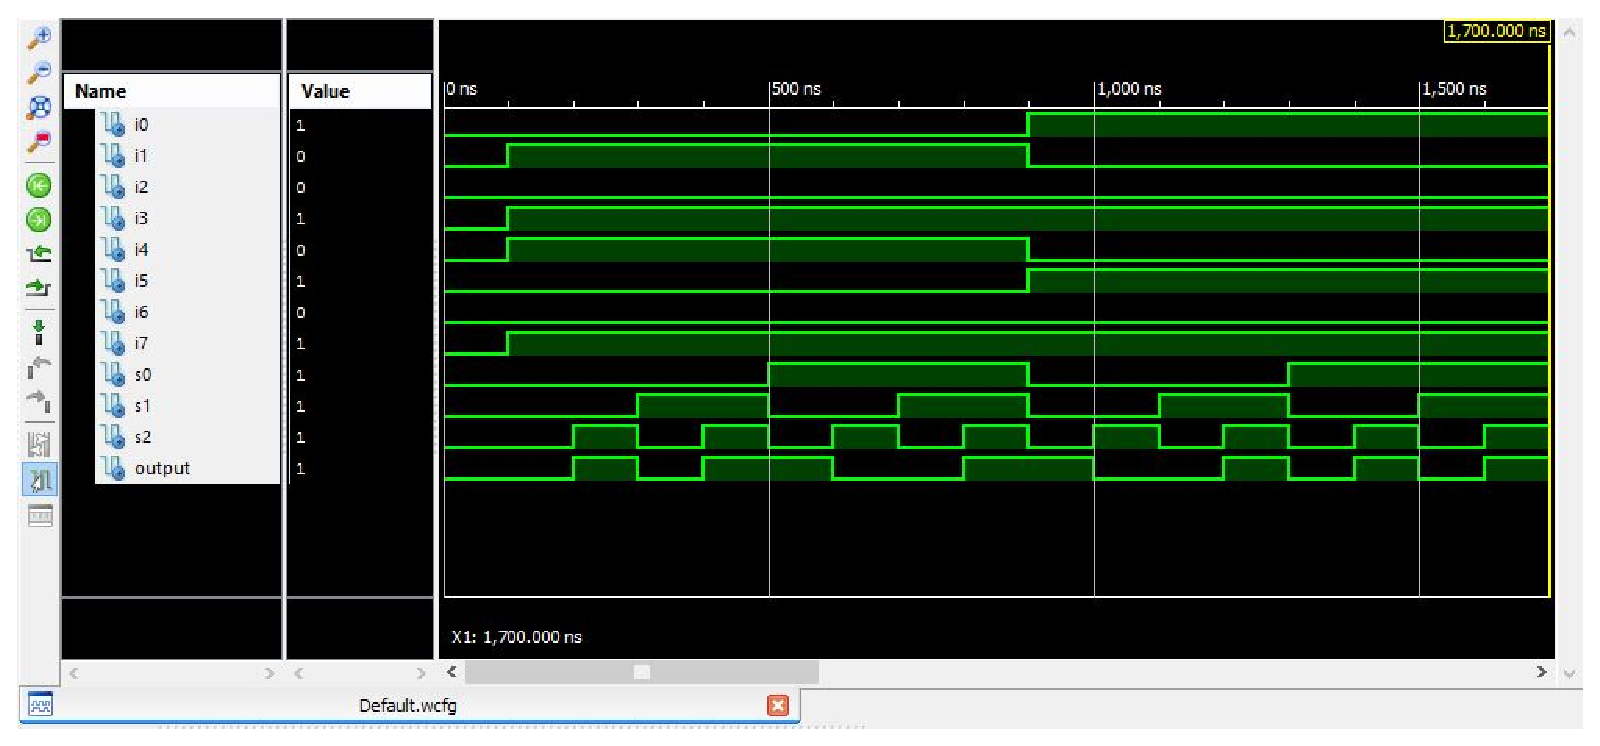
\includegraphics[scale=0.7]{mux}
\caption{Timing Diagram for 8x1 multiplexer from 0ns to 1700 ns}
\label{fig1}
\end{figure}
\begin{figure}[!ht]
\centering
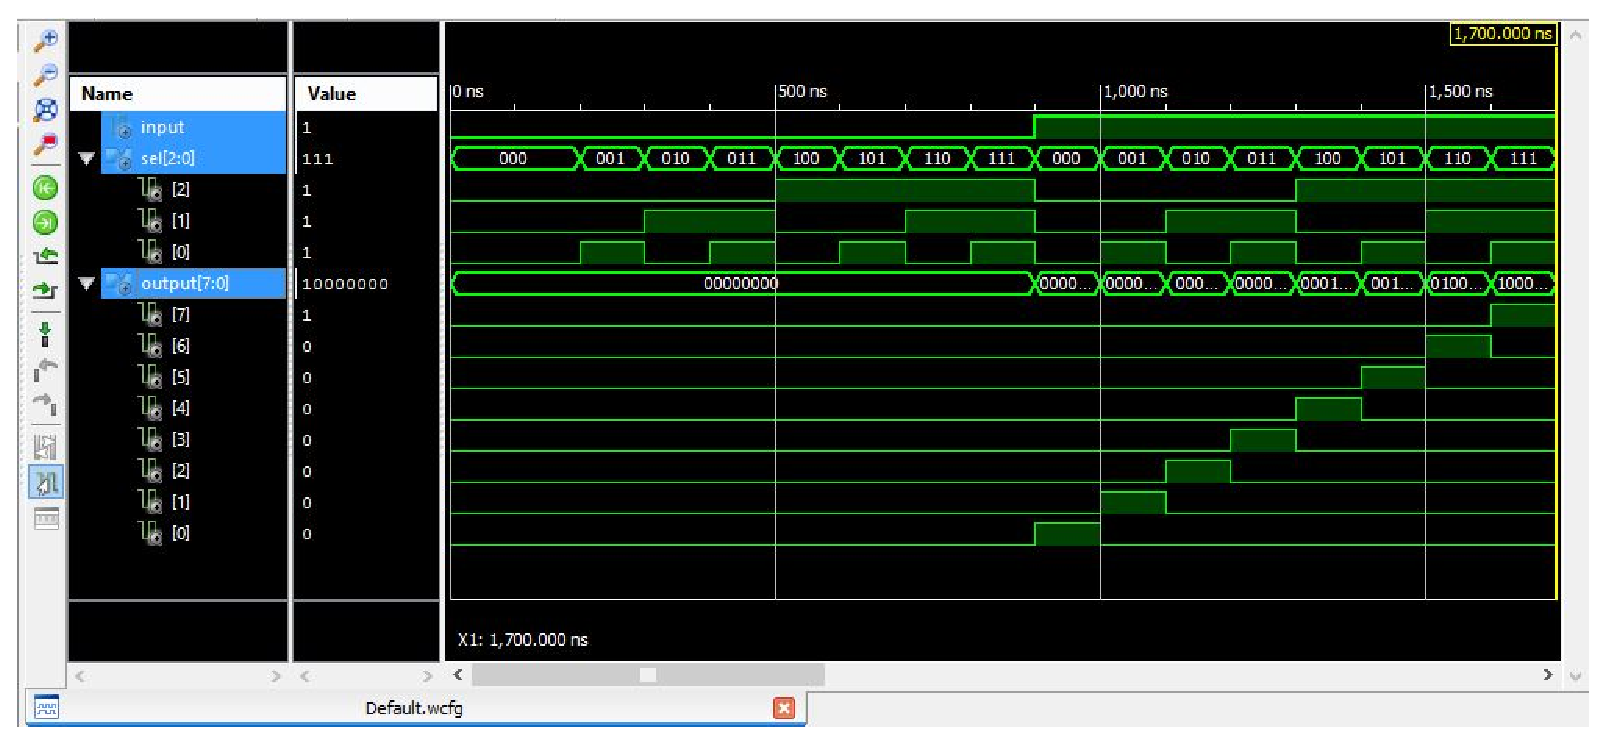
\includegraphics[scale=0.7]{demux}
\caption{Timing Diagram for 1x8 demultiplexer from 0ns to 1700 ns}
\label{fig2}
\end{figure}
\section{Codes}
Here I have include working code for both multiplexer and demultiplexer
\subsection{code for multiplexer}
\begin{lstlisting}[style=vhdl]
-----------------------------------------------------------------------
-- Company: 
-- Engineer: 
-- 
-- Create Date:    14:28:18 02/11/2014 
-- Design Name: 
-- Module Name:    multiplexer - Behavioral 
-- Project Name: 
-- Target Devices: 
-- Tool versions: 
-- Description: 
--
-- Dependencies: 
--
-- Revision: 
-- Revision 0.01 - File Created
-- Additional Comments: 
--
-----------------------------------------------------------------------
library IEEE;
use IEEE.STD_LOGIC_1164.ALL;

-- Uncomment the following library declaration if using
-- arithmetic functions with Signed or Unsigned values
--use IEEE.NUMERIC_STD.ALL;

-- Uncomment the following library declaration if instantiating
-- any Xilinx primitives in this code.
--library UNISIM;
--use UNISIM.VComponents.all;

entity multiplexer is
    Port ( i0 : in  STD_LOGIC;
           i1 : in  STD_LOGIC;
           i2 : in  STD_LOGIC;
           i3 : in  STD_LOGIC;
           i4 : in  STD_LOGIC;
           i5 : in  STD_LOGIC;
           i6 : in  STD_LOGIC;
           i7 : in  STD_LOGIC;
           s0 : in  STD_LOGIC;
           s1 : in  STD_LOGIC;
           s2 : in  STD_LOGIC;
           output : out  STD_LOGIC);
end multiplexer;

architecture Behavioral of multiplexer is

begin
output <= i0 when s0 = '0' and s1 = '0' and s2 = '0' else 
	  i1 when s0 = '0' and s1 = '0' and s2 = '1' else 
	  i2 when s0 = '0' and s1 = '1' and s2 = '0' else  
	  i3 when s0 = '0' and s1 = '1' and s2 = '1' else
	  i4 when s0 = '1' and s1 = '0' and s2 = '0' else
	  i5 when s0 = '1' and s1 = '0' and s2 = '1' else
	  i6 when s0 = '1' and s1 = '1' and s2 = '0' else
	  i7 when s0 = '1' and s1 = '1' and s2 = '1' ;
end Behavioral;


\end{lstlisting}
\newpage
\subsection{Code for Demultiplexer}
\begin{lstlisting}[style=vhdl]
-----------------------------------------------------------------------
-- Company: 
-- Engineer: 
-- 
-- Create Date:    15:32:55 02/11/2014 
-- Design Name: 
-- Module Name:    demux - Behavioral 
-- Project Name: 
-- Target Devices: 
-- Tool versions: 
-- Description: 
--
-- Dependencies: 
--
-- Revision: 
-- Revision 0.01 - File Created
-- Additional Comments: 
--
-----------------------------------------------------------------------
library IEEE;
use IEEE.STD_LOGIC_1164.ALL;

-- Uncomment the following library declaration if using
-- arithmetic functions with Signed or Unsigned values
--use IEEE.NUMERIC_STD.ALL;

-- Uncomment the following library declaration if instantiating
-- any Xilinx primitives in this code.
--library UNISIM;
--use UNISIM.VComponents.all;

entity demux is
    Port ( input : in  STD_LOGIC;
           sel : in  STD_LOGIC_VECTOR (2 downto 0);
           output : out  STD_LOGIC_VECTOR (7 downto 0));
end demux;

architecture Behavioral of demux is
begin process (input, sel)
begin
output <= "00000000";
	case sel is 
		when "000" =>
			output(0) <= input;
		when "001" =>
			output(1) <= input;
		when "010" =>
			output(2) <= input;
		when "011" =>
			output(3) <= input;
		when "100" =>
			output(4) <= input;
		when "101" =>
			output(5) <= input;
		when "110" =>
			output(6) <= input;
		when "111" =>
			output(7) <= input;
		when others =>
			null;
	end case;
end process;
end Behavioral;


\end{lstlisting}
\section{Inference}
In this assignment I infered the followings:\\
\verb|1.| Working of 8x1 multiplexer and 1x8 demultiplexers \\
\verb|2.| Wrinting VHDL code in behavioral style rather then structural style \\
\verb|3.| Working with Logic Vectors in VHDL \\
\verb|4.| Use of select lines with multplexers and demultiplexer \\
\verb|5.| Use of select lines as decoders \\
\end{document}
